%% Согласно ГОСТ Р 7.0.11-2011:
%% 5.3.3 В заключении диссертации излагают итоги выполненного исследования, рекомендации, перспективы дальнейшей разработки темы.
%% 9.2.3 В заключении автореферата диссертации излагают итоги данного исследования, рекомендации и перспективы дальнейшей разработки темы.

\begin{enumerate}
\begin{samepage}
    \item Проведён всесторонний анализ современных методов моделирования и выявления компьютерных атак. Выявлены ключевые недостатки существующих подходов: низкая интерпретируемость моделей машинного обучения, статичность графов атак, неспособность деревьев атак масштабироваться на сложные сценарии, а также высокий уровень ложных срабатываний при аномальном анализе. Обоснован выбор атрибутивных метаграфов в качестве основы для новой методики, что впервые предложено в работе~\cite{Latypov2020} и развито в~\cite{inside2026}.
\end{samepage}
    \item Формализована модель атрибутивного метаграфа в контексте кибербезопасности. Введены определения вершин, гипердуг, атрибутов и операций алгебры метаграфов (объединение, композиция, проекция). Показано, что такая модель естественным образом отражает многообъектные действия злоумышленника и допускает интеграцию с~таксономией MITRE~ATT\&CK. Модель реализует \textbf{многоуровневую структуру} (стратегический, тактический, методический уровни), впервые описанную в~\cite{Latypov2020} и визуализированную на Рис.~\ref{fig:multilevel}. 

% Рисунок 1: Многоуровневая модель
\begin{figure}[ht]
\centering
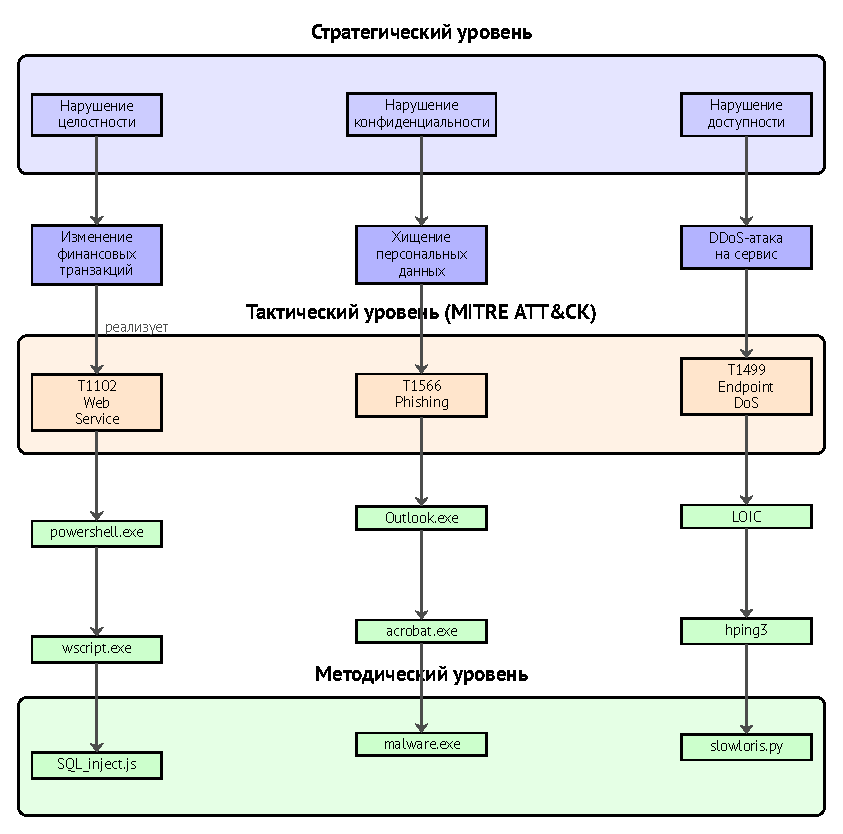
\includegraphics[width=0.85\textwidth]{images/fig_multilevel_metagraph}
\caption{Многоуровневая атрибутивная метаграфовая модель}
\label{fig:multilevel}
\end{figure}

    \item Разработана методика выявления атак, включающая архитектуру системы AMGD (Рис.~\ref{fig:siem}), алгоритм сопоставления эталонных и динамических метаграфов, а также механизм оценки риска компрометации на~основе взвешенных путей и вероятностей реализации. Предложенный алгоритм учитывает семантическое сходство атрибутов и временные окна, что повышает точность обнаружения. 
    
        % Рисунок 2: Многоуровневая модель
        \begin{figure}[ht]
        \centering
        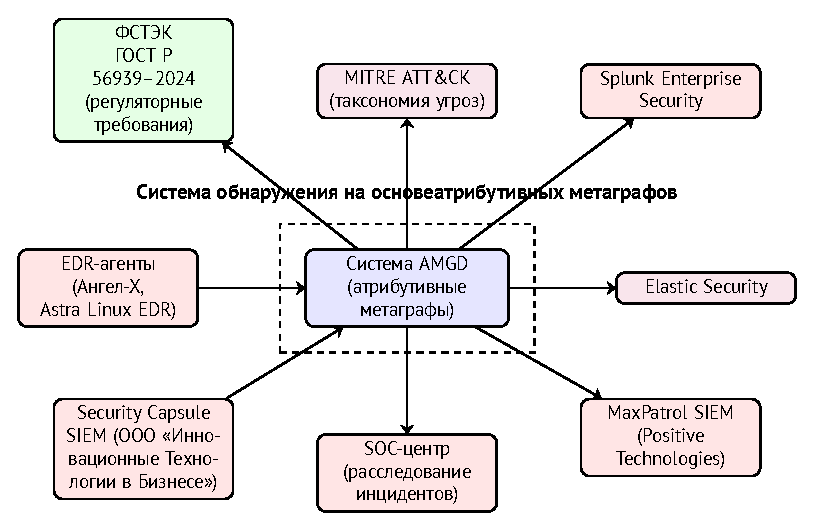
\includegraphics[width=0.85\textwidth]{images/fig_siem_integration}
        \caption{Интеграция с SIEM/SOAR}
        \label{fig:siem}
        \end{figure}

    \item Реализован прототип программной системы и проведено имитационное моделирование на данных реальных APT-кампаний (TAO, Unit 8200) и~финансово мотивированных группировок (FIN7). Экспериментальная оценка, описанная в~\cite{inside2026} и дополненная в~\cite{Latypov2025}, показала, что предложенный подход обеспечивает F1-score = 0.86, что на 22\%~выше, чем у лучших базовых методов (Таблица~\ref{tab:results}), при уровне ложных срабатываний 1.3\%.

    \item Подтверждена практическая применимость методики в пилотном проекте SOC-центра ПАО «Транснефть», где за три месяца тестирования система выявила 12 инцидентов, пропущенных стандартными правилами корреляции. Результаты согласуются с~данными, представленными в~\cite{Latypov2025}, где отмечено снижение ложных срабатываний на 19–23\%.
\end{enumerate}

Разработанная методика может быть рекомендована к~внедрению в~SIEM/SOAR-платформы (Splunk, Elastic Security, QRadar) в~качестве модуля контекстного обогащения. Она также подходит для сертификации в~соответствии с~требованиями ФСТЭК России и~ГОСТ~Р~56939–2024, поскольку обеспечивает интерпретируемость алертов и~связь технических артефактов с~бизнес-последствиями.

Перспективы дальнейшей разработки включают:
\begin{itemize}
    \item интеграцию с~фреймворком MITRE D3FEND для автоматической генерации рекомендаций по реагированию;
    \item поддержку онтологий STIX~2.1/TAXII для совместимости с~платформами обмена угрозами;
    \item внедрение механизмов самообучения на~основе больших языковых моделей (LLM) для полуавтоматического расширения библиотеки эталонных паттернов.
\end{itemize}